\documentclass[journal,5pt,twocolumn]{IEEEtran}
%\makeatletter
\usepackage{tikz}
\usetikzlibrary{shapes,arrows}
\makeatother
\usepackage{setspace}
\usepackage{gensymb}
\usepackage{xcolor}
\usepackage{caption}
%\usepackage{stackengine}
%\usepackage{subcaption}
%\doublespacing
\usepackage{xcolor}
\usepackage{lipsum}
\singlespacing
\def\baselinestretch{1.5}
\usepackage{fancyhdr}
\pagestyle{fancy}
\fancyhf{} 

%\counterwithin{enumi}{section}
%\counterwithin{equation}{enumi}
%\counterwithin{figure}{enumi}

\newcommand\figref{Fig.~\ref}
\usepackage[colorlinks=true, allcolors=black]{hyperref}

\usepackage{graphicx}
%\graphicspath{ {./images}  }
%\usepackage{amssymb}
%\usepackage{relsize}
\usepackage[cmex10]{amsmath}
\usepackage{mathtools}
%\usepackage{amsthm}
\interdisplaylinepenalty=2500
%\savesymbol{iint}
%\usepackage{txfonts}
%\restoresymbol{TXF}{iint}
\usepackage{wasysym}
\usepackage{amsthm}
\usepackage{mathrsfs}
\usepackage{txfonts}
\usepackage{stfloats}
\usepackage{cite}
\usepackage{cases}
\usepackage{mathtools}
\usepackage{subfig}
\usepackage{enumerate}	
\usepackage{enumitem}
\usepackage{amsmath}
%\usepackage{xtab}
\usepackage{longtable}
\usepackage{multirow}
%\usepackage{algorithm}
%\usepackage{algpseudocode}
\usepackage{enumitem}
\usepackage{mathtools}
%\usepackage{iithtlc}
\usepackage{tikz}
\usetikzlibrary{shapes,arrows}
%\usetikzlibrary{arrows.meta,calc,positioning}
%\usepackage[framemethod=tikz]{mdframed}
\usepackage{listings}
    \usepackage[latin1]{inputenc}                                 %%
    \usepackage{color}                                            %%
    \usepackage{array}                                            %%
    \usepackage{longtable}                                        %%
    \usepackage{calc}                                             %%
    \usepackage{multirow}                                         %%
    \usepackage{hhline}                                           %%
    \usepackage{ifthen}                                           %%
  %optionally (for landscape tables embedded in another document): %%
    \usepackage{lscape}     


%\usepackage{stmaryrd}


%\usepackage{wasysym}
%\newcounter{MYtempeqncnt}
\DeclareMathOperator*{\Res}{Res}
%\renewcommand{\baselinestretch}{4}
%\setcounter{secnumdepth}{4}
\renewcommand\thesection{\arabic{section}}
\renewcommand\thesubsection{\thesection.\arabic{subsection}}
\renewcommand\thesubsubsection{\thesubsection.\arabic{subsubsection}}
%\renewcommand\thesubsubsubsection{\thesubsubsection.\arabic{subsubsubsection}}

%\renewcommand\thesectiondis{\arabic{section}}
%\renewcommand\thesubsectiondis{\thesectiondis.\arabic{subsection}}
%\renewcommand\thesubsubsectiondis{\thesubsectiondis.\arabic{subsubsection}}
%\renewcommand\thesubsubsubsectiondis{\thesubsubsectiondis.\arabic{subsubsubsection}}
% correct bad hyphenation here
\hyphenation{Future Wireless communications}

%\lstset{
%language=C,
%frame=single, 
%breaklines=true
%}

%\lstset{
	%%basicstyle=\small\ttfamily\bfseries,
	%%numberstyle=\small\ttfamily,
	%language=Octave,
	%backgroundcolor=\color{white},
	%%frame=single,
	%%keywordstyle=\bfseries,
	%%breaklines=true,
	%%showstringspaces=false,
	%%xleftmargin=-10mm,
	%%aboveskip=-1mm,
	%%belowskip=0mm
%}

%\surroundwithmdframed[width=\columnwidth]{lstlisting}
\def\inputGnumericTable{}                                 %%

\lstset{
%language=python,
frame=single, 
breaklines=true,
columns=fullflexible
}

 \usepackage{watermark}

\begin{document}
%
\tikzstyle{block} = [rectangle, draw,
text width=7em, text centered, minimum height=4em]
\tikzstyle{sum} = [draw, circle, node distance=3cm]
\tikzstyle{input} = [coordinate]
\tikzstyle{output} = [coordinate]
\tikzstyle{pinstyle} = [pin edge={to-,thin,black}]
\tikzstyle{line} = [draw, -latex']
\theoremstyle{definition}
\newtheorem{theorem}{Theorem}[section]
\newtheorem{problem}{Problem}
\newtheorem{proposition}{Proposition}[section]
\newtheorem{lemma}{Lemma}[section]
\newtheorem{corollary}[theorem]{Corollary}
\newtheorem{example}{Example}[section]
\newtheorem{definition}{Definition}[section]
%\newtheorem{algorithm}{Algorithm}[section]
%\newtheorem{cor}{Corollary}
\newcommand{\BEQA}{\begin{eqnarray}}
\newcommand{\EEQA}{\end{eqnarray}}
\newcommand{\define}{\stackrel{\triangle}{=}}
\bibliographystyle{IEEEtran}
%\bibliographystyle{ieeetr}
\providecommand{\nCr}[2]{\,^{#1}C_{#2}} % nCr
\providecommand{\nPr}[2]{\,^{#1}P_{#2}} % nPr
\providecommand{\mbf}{\mathbf}
\providecommand{\pr}[1]{\ensuremath{\Pr\left(#1\right)}}
\providecommand{\qfunc}[1]{\ensuremath{Q\left(#1\right)}}
\providecommand{\sbrak}[1]{\ensuremath{{}\left[#1\right]}}
\providecommand{\lsbrak}[1]{\ensuremath{{}\left[#1\right.}}
\providecommand{\rsbrak}[1]{\ensuremath{{}\left.#1\right]}}
\providecommand{\brak}[1]{\ensuremath{\left(#1\right)}}
\providecommand{\lbrak}[1]{\ensuremath{\left(#1\right.}}
\providecommand{\rbrak}[1]{\ensuremath{\left.#1\right)}}
\providecommand{\cbrak}[1]{\ensuremath{\left\{#1\right\}}}
\providecommand{\lcbrak}[1]{\ensuremath{\left\{#1\right.}}
\providecommand{\rcbrak}[1]{\ensuremath{\left.#1\right\}}}
\theoremstyle{remark}
\newtheorem{rem}{Remark}
\newcommand{\sgn}{\mathop{\mathrm{sgn}}}
\providecommand{\abs}[1]{\left\vert#1\right\vert}
\providecommand{\res}[1]{\Res\displaylimits_{#1}} 
\providecommand{\norm}[1]{\lVert#1\rVert}
\providecommand{\mtx}[1]{\mathbf{#1}}
\providecommand{\mean}[1]{E\left[ #1 \right]}
\providecommand{\fourier}{\overset{\mathcal{F}}{ \rightleftharpoons}}
%\providecommand{\hilbert}{\overset{\mathcal{H}}{ \rightleftharpoons}}
\providecommand{\system}{\overset{\mathcal{H}}{ \longleftrightarrow}}
	%\newcommand{\solution}[2]{\textbf{Solution:}{#1}}
\newcommand{\solution}{\noindent \textbf{Solution: }}
\newcommand{\myvec}[1]{\ensuremath{\begin{pmatrix}#1\end{pmatrix}}}
\providecommand{\dec}[2]{\ensuremath{\overset{#1}{\underset{#2}{\gtrless}}}}
\DeclarePairedDelimiter{\ceil}{\lceil}{\rceil}
%\numberwithin{equation}{subsection}
\numberwithin{equation}{section}
%\numberwithin{problem}{subsection}
%\numberwithin{definition}{subsection}
%\makeatletter
%\@addtoreset{figure}{section}
%\makeatother
\let\StandardTheFigure\thefigure
%\renewcommand{\thefigure}{\theproblem.\arabic{figure}}
%\renewcommand{\thefigure}{\thesection}
%\numberwithin{figure}{subsection}
%\numberwithin{equation}{subsection}
%\numberwithin{equation}{section}
%\numberwithin{equation}{problem}
%\numberwithin{problem}{subsection}
%\numberwithin{problem}{section}
%%\numberwithin{definition}{subsection}
%\makeatletter
%\@addtoreset{figure}{problem}
%\makeatother
%\makeatletter
%\@addtoreset{table}{problem}
%\makeatother
\let\StandardTheFigure\thefigure
\let\StandardTheTable\thetable
\let\vec\mathbf
%%\renewcommand{\thefigure}{\theproblem.\arabic{figure}}
%\renewcommand{\thefigure}{\theproblem}
%%\numberwithin{figure}{section}
%%\numberwithin{figure}{subsection}
\def\putbox#1#2#3{\makebox[0in][l]{\makebox[#1][l]{}\raisebox{\baselineskip}[0in][0in]{\raisebox{#2}[0in][0in]{#3}}}}
     \def\rightbox#1{\makebox[0in][r]{#1}}
     \def\centbox#1{\makebox[0in]{#1}}
     \def\topbox#1{\raisebox{-\baselineskip}[0in][0in]{#1}}
     \def\midbox#1{\raisebox{-0.5\baselineskip}[0in][0in]{#1}}
\title{ 
%	\logo{
FREQUENCY MODULATION
%	}
}
\author{ Under guidance of Dr. GVV SHARMA}% <-this % stops a space
\thiswatermark{\centering \put(-50,-105){
\includegraphics[scale=0.5]{iith.png}}}
% make the title area
\maketitle
\tableofcontents
\section{\textbf{Introduction}}
Frequency modulation (FM) is a widely used technique in modern communication systems. It is a form of modulation that encodes information by varying the frequency of a carrier signal in proportion to the message signal\\
One important parameter in FM is the bandwidth, which determines the range of frequencies required to accurately represent the modulated signal. The Carson's rule provides a simple approximation for the bandwidth of an FM signal.In this the bandwidth of an FM signal can be calculated by analyzing its frequency spectrum using techniques such as Fourier analysis.
\section{\textbf{Bandwidth Calculation}}
\subsection{\textbf{Bandwidth calculation method}}

Bandwidth refers to the range of frequencies over which a signal or system operates. There are several methods to calculate the bandwidth of a signal, including the 3dB attenuation method and the spectral density method.\\
\begin{enumerate}
\item  The 3dB attenuation method involves finding the frequency range where the signal's power or amplitude is reduced by half (-3dB) from its maximum value.However, it does not take into account the full frequency spectrum of the signal or system, and may not accurately reflect the actual bandwidth of the signal.
\item The spectral density method calculates the bandwidth of a signal or system by analyzing its frequency content. Specifically, it calculates the power spectral density (PSD) of the signal or system, which is a measure of how the power of the signal is distributed across different frequencies. The bandwidth is then defined as the frequency range over which 99\%of the total power is contained.\\
 This method provides a more accurate and comprehensive measure of bandwidth as it takes into account the entire frequency spectrum of the signal or system.
\end{enumerate}

\subsection{\textbf{Steps for Generating Frequency Modulated (FM) Signal:}}
   

\begin{enumerate}
\item Loading the Audio File:  Load the WAV file containing the audio input signal.
The audio input signal is a time-varying signal, and we need to convert it into the frequency domain to analyze its bandwidth.

\item Computing the Fourier Transform:
The Fast Fourier Transform (FFT) is a numerical algorithm that computes the Discrete Fourier Transform (DFT) of a sequence. The FFT is an efficient way to calculate the frequency spectrum of a signal. Apply the FFT to the audio input signal to obtain its frequency spectrum.The spectrum of input audio signal is plotted in \figref{fig:input_spectrum}
\begin{figure}
\centering 
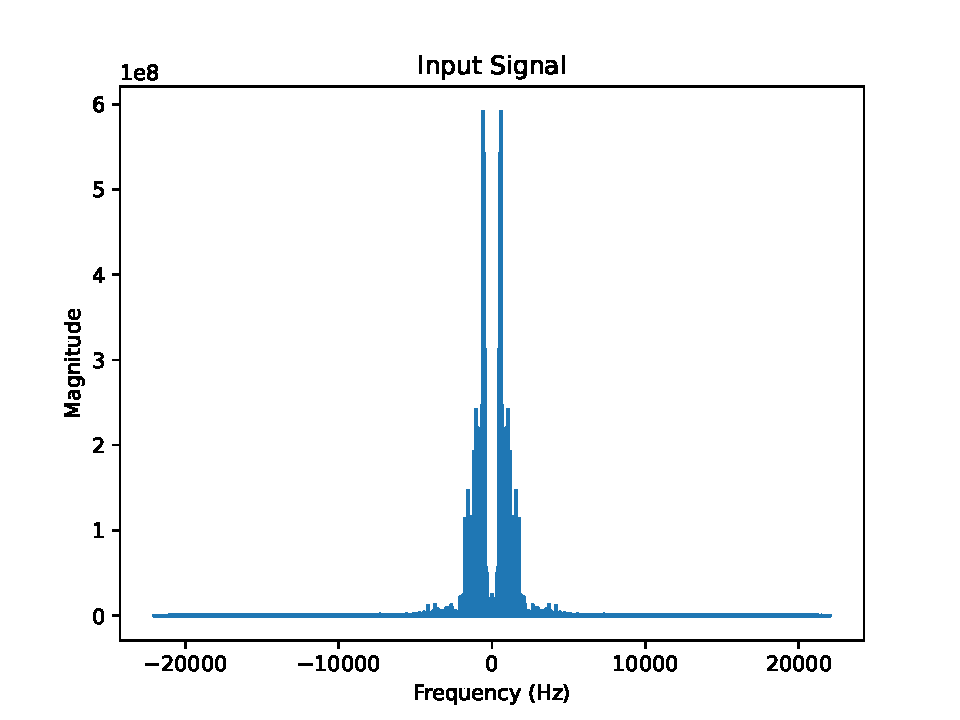
\includegraphics[width=\columnwidth]{./inputs.pdf}
\caption{spectrum analysis of input signal}
\label{fig:input_spectrum}
\end{figure}


\begin{align*}
X(f) = FFT(x(t))
\end{align*}
Where X(f) is the frequency representation of the signal, x(t) is the input signal
\item Calculating the frequency Range: Calculates the frequencies for each sample in the audio signal. The frequency range is used to plot the magnitude spectrum of the audio signal.

\item Calculating the Power Spectral Density: PSD is the power of the signal per unit of frequency. The PSD is calculated by squaring the absolute value of the FFT.
\begin{align*}
PSD(f)=\lvert X(f) \rvert^2 
\end{align*}
Where PSD(f) is the power spectral density at frequency f, X(f) is the Fourier Transform of the input signal

\item Finding the Frequency Range with Significant Power:
The frequency range with significant power in the PSD of the FM signal. This can be done by creating a mask that identifies frequencies where the PSD is greater than a certain threshold. Let's denote the threshold as T. Then the mask can be defined as:
\begin{align*}
mask(f) &=
\begin{cases}
 1 \quad PSD(f) > T\\
0 \quad otherwise
\end{cases}
\end{align*}

\item Calculating the Bandwidth: Calculate the bandwidth as the difference between the maximum and minimum frequencies in the range with significant power.
\begin{align*}
B = f_u - f_l
\end{align*}
where $f_l $ and $f_u $arethe lower and upper frequency bounds of the range  respectively.0
 \item Frequency modulation to the sound signal:
 
 \begin{equation}
 c(t) = A_c \cos(2 \pi F_c t )
 \label{eq:carrier_signal} 
 \end{equation}
 Equation \ref{eq:carrier_signal} shows the mathematical expression for a carrier signal with amplitude $A_c$, frequency $F_c$. 
 
 The frequency modulation is applied to the sound signal using the formula
 \begin{equation}
 s(t) = A_c \cos \left(2 \pi F_c t + K_{f} \int_{0}^t m(\tau) d\tau \right) 
 \end{equation}

 where $A_c$ is the amplitude of the carrier signal, $F_c$ is the frequency of the carrier signal, $m(t)$ is the modulating signal, $K_{f}$ is the frequency sensitivity constant of the modulating signal.
 \begin{align*}
K_{f} = \frac{\Delta f}{A_m} 
 \end{align*}
 
 \begin{figure}
\centering 
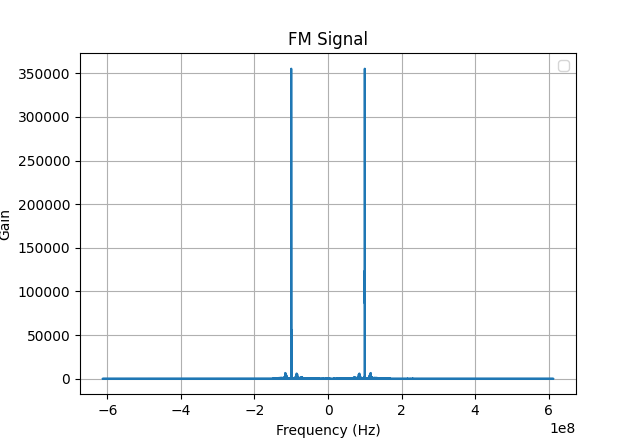
\includegraphics[width=\columnwidth]{./fm.png}
\caption{spectrum analysis of fm signal}
\label{fig:fm_spectrum}
\end{figure}

 The bandwidth of the FM signal generated using a carrier frequency of 100 MHz and frequency sensitivity of 25 kHz is approximately 7 kHz. This was calculated by finding the spectral density of the FM signal using the Fourier transform.
The spectrum of FM signal is plotted in \figref{fig:fm_spectrum} using below code
\begin{center}
\fcolorbox{red}{white}{\parbox{12.5cm}
{\href{https://github.com/Gangagopinath/fwc/tree/main/FM/code}
{/codes/mod.py}}}
\end{center}

\end{enumerate}




\section{\textbf{Result}}
Generate a FM signal from an audio signal with a bandwidth of 7 KHz.The bandwidth for both FM and audio signal is a calculated using power spectral density.\figref{fig:fm_spectrum} shows the spectrum of FM signal



\end{document}